\documentclass{article}

\usepackage{PRIMEarxiv}

\usepackage[utf8]{inputenc} % allow utf-8 input
\usepackage[T1]{fontenc}    % use 8-bit T1 fonts
\usepackage{hyperref}       % hyperlinks
\usepackage{url}            % simple URL typesetting
\usepackage{booktabs}       % professional-quality tables
\usepackage{amsfonts}       % blackboard math symbols
\usepackage{nicefrac}       % compact symbols for 1/2, etc.
\usepackage{microtype}      % microtypography
\usepackage{fancyhdr}       % header
\usepackage{graphicx}       % graphics
\usepackage{amsmath,amssymb,amsthm,xcolor,enumitem,caption,float}
\usepackage{algorithm,algpseudocode,needspace,array}
\hypersetup{colorlinks=true,linkcolor=blue!50!black,citecolor=blue!50!black,urlcolor=blue!50!black}
% figures are produced by experiments.py into ../results/figures/ (on Overleaf they can also go in media/)
\graphicspath{{../results/figures/}{media/}}

\setlist{nosep,leftmargin=*}
\captionsetup{font=small,labelfont=bf}
\newtheorem{definition}{Definition}
\newtheorem{proposition}{Proposition}

%Header
\pagestyle{fancy}
\thispagestyle{empty}
\rhead{ \textit{ }}
\chead{}
\fancyhead[LO]{Coordinating Crowds: Congestion, Information and Correlated Equilibrium}

\renewcommand{\undertitle}{Final Report \;|\; Foundations of AI -- Multi-Agent Systems \;|\; IIT Gandhinagar}

%% Title
\title{Coordinating Crowds at Shared Facilities: Congestion Games, Information Design and Correlated Equilibrium
\thanks{\textit{\underline{Code and data generator}}: \url{https://github.com/YashG1836/crowd-congestion};
\textit{\underline{live demo}}: \url{https://crowd-congestion.streamlit.app/}.
Every figure and number in this report is produced by \texttt{python experiments.py}.}}

\author{
  Harsh Kumar Jha \\ 24110130
  \And
  Yash Goyal \\ 24110399
  \And
  Piyush Kumar Keshri \\ 24110260
  \And
  Garv Singhal \\ 24110119
}
\date{}

\begin{document}
\raggedbottom
\maketitle

\begin{abstract}
\noindent Many people share one bottleneck and each chooses \emph{when} to use it: cars at a bridge, backups on a network
link, diners at a food court, students at a hostel mess. We model this as an atomic congestion game over time slots
with a fluid queue, and treat the crowd display as an \emph{information designer}. We (i)~compute Nash equilibria,
the social optimum and the price of anarchy (PoA) for five domains and 24 synthetic mess instances (4 messes, 3000
students, 3 meals); (ii)~simulate day-to-day play under nine information policies and three behaviour regimes; and
(iii)~study private recommendations as \emph{correlated equilibria} (CE). Selfish timing costs 3--8$\times$ the
optimum. An exact live counter that everyone reacts to raises the cost about 5$\times$ (the El Farol effect).
Recommendations drawn from a Nash schedule are obeyed, stable and remove herding once 50--70\% of students use
them, but we prove and verify by linear programming that advice alone cannot beat Nash in a large crowd. The CE
obedience constraints, however, give the smallest reward that makes the optimum self-enforcing: rewards worth
about 2.7 minutes for 13\% of students cut the average cost from 2.24 to 0.36 minutes.
\end{abstract}

\keywords{Congestion games \and Correlated equilibrium \and Information design \and Price of anarchy \and No-regret learning}

% ============================================================================
\section{Introduction}
Congestion at a shared facility is usually a \emph{coordination} problem, not a capacity problem. On a popular
night the IITGN mess is packed at 20:00--20:30 and almost empty after 21:00, yet the counter could serve everyone
over the two hours. The same structure appears on roads (everyone wants to cross a bridge just before 9:00), in
networks (laptops all back up at 22:00), in restaurants and in gyms. Every person who joins a queue delays everyone
behind them but feels only their own wait.

A live crowd counter, easy to build from the QR scans the mess already records, looks like the obvious fix. But in
the El Farol bar problem~\cite{arthur} people who react to the same forecast move together, and a counter could
make the rush jump between slots. Our central question is: \emph{what should a display show, how fresh and how
accurate should it be, and to whom, so that people's own choices lead to short waits?} Following our advisor's
suggestion we treat congestion in general, use the correlated equilibrium~\cite{aumann} as the main solution
concept for ``telling different people different things'', and use the mess as a detailed case study with
synthetic data.

\textbf{Contributions.} (1)~One slot-congestion model and solver suite (Nash, Wardrop, optimum, PoA) covering
roads, networks, restaurants, gyms and the mess. (2)~A day-to-day simulator comparing nine information policies
under three behaviour models and three learning rules. (3)~A population-scale treatment of correlated
recommendations: a fair shuffled recommender, a proof that advice cannot beat Nash in large monotone games, a
best-CE linear program, and the \emph{price of obedience}. (4)~A synthetic semester of QR-scan logs with
calibration and nowcasting. Every number below is produced by \texttt{python experiments.py}.

% ============================================================================
\section{Preliminaries}
\begin{definition}[Game, NE] Players $i$ choose actions $s_i$; $c_i(s)$ is $i$'s cost. A profile is a
\emph{Nash equilibrium} (NE) if no player can lower their cost by changing only their own action~\cite{nash}.
Congestion games have pure NE because they admit a potential~\cite{rosenthal}.\end{definition}
\begin{definition}[CE and CCE~\cite{aumann}] A mediator draws $s\sim p$ and privately tells each player $s_i$.
$p$ is a \emph{correlated equilibrium} if for all $i$ and actions $a,a'$:
$\sum_{s:s_i=a}p(s)\,[c_i(s)-c_i(a',s_{-i})]\le 0$. It is a \emph{coarse} CE if for all $i,a'$:
$\sum_s p(s)\,[c_i(s)-c_i(a',s_{-i})]\le0$. NE$\subset$CE$\subset$CCE, and both sets are polytopes, so the best
one is a linear program.\end{definition}
\begin{definition}[PoA] With social cost $SC=\sum_i c_i$, $\mathrm{PoA}=SC(\text{worst NE})/SC(\text{optimum})$;
the price of stability uses the best NE~\cite{koutsoupias,roughgarden}.\end{definition}
\begin{definition}[Incomplete information, learning] In a Bayesian game players do not know a state $\omega$ and
best-respond in expectation (Bayesian NE)~\cite{harsanyi}. In logit response a slot is chosen with probability
$\propto e^{-\lambda\,\text{cost}}$~\cite{mckelvey}. Hedge~\cite{freund} (full feedback) and EXP3~\cite{auer}
(bandit feedback) have no external regret, so joint play approaches the CCE set; regret matching~\cite{hart} has
no swap regret and approaches the CE set.\end{definition}

\textbf{Three small games} (Table~\ref{tab:toy}, Fig.~\ref{fig:theory}). \emph{Pigou's network:} with a peak road
costing $x^p$ and an alternative costing 1, $\mathrm{PoA}(p)=[1-p(p+1)^{-(p+1)/p}]^{-1}$ (4/3 at $p{=}1$, 2.15
at $p{=}4$). \emph{Two-student dinner game:} Peak costs the number of students there, Late costs 1.5; the shared
counter makes both students alternate between (Peak, Peak) and (Late, Late); a private fair coin is a CE that
reaches the optimum. \emph{Intersection (Chicken):} utilities 6/6, 2/7, 7/2, 0/0; the best CE ($\frac12$ Stop--Stop,
$\frac14$ each Stop--Go, Go--Stop) gives \textbf{5.25} to each driver, more than any mixture of Nash equilibria (4.67).

\begin{table}[H]\centering\small
\caption{Two-student dinner game: what each kind of information achieves (computed by \texttt{theory.py}).}\label{tab:toy}
\begin{tabular}{lcc}\toprule
Policy & Total cost & Ratio to optimum\\\midrule
Shared live counter (both react to yesterday) & 3.5 & 1.40\\
No information (symmetric mixed NE, Peak w.p.\ 1/2) & 3.0 & 1.20\\
Private fair coin = correlated equilibrium & \textbf{2.5} & \textbf{1.00}\\\bottomrule
\end{tabular}\end{table}

% ============================================================================
\section{Problem formulation}
\textbf{Players and slots.} $n$ people, $T$ slots of $\Delta$ minutes (mess: $T{=}12$, $\Delta{=}10$). Person $i$
has a private preferred slot $\tau_i$ and flexibility $\beta_i$ (minutes of waiting they would accept to avoid
moving one slot). People with equal $(\tau,\beta)$ form a \emph{type} $k$; the state is $X[k,t]$, the number of
type-$k$ people in slot $t$, with loads $A_t=\sum_k X[k,t]$. The cost of a type-$k$ person in slot $t$ is
\begin{equation}
c_k(t;A)=g_t(A)+\beta_k\,|t-\tau_k|,\qquad SC(X)=\sum_t A_t\,g_t(A)+\sum_{k,t}X[k,t]\,\beta_k|t-\tau_k|.
\end{equation}
\textbf{Fluid queue.} One counter serves $\mu$ people per minute, arrivals are spread evenly within a slot,
service is first come first served, and leftover queue carries over. With backlog $q_0$ and net rate
$r=(A_t-\mu\Delta)/\Delta$, the queue after $u$ minutes is $\max(0,q_0+ru)$ and an arrival then waits that divided
by $\mu$. Averaging over the slot,
\begin{equation}
W_t=\begin{cases}\big(q_0+\tfrac{A_t-\mu\Delta}{2}\big)/\mu & r\ge0\\[2pt]
\big(q_0 s+\tfrac{r s^2}{2}\big)/(\Delta\mu),\; s=\min(\Delta,q_0/(-r)) & r<0\end{cases},\qquad q_0^{\text{next}}=\max(0,q_0+A_t-\mu\Delta).
\end{equation}
Total waiting $\sum_tA_tW_t$ equals the area under the queue (Little's law). This is Vickrey's bottleneck
model~\cite{vickrey} for roads and a deterministic link buffer for networks. We use $g_t=W_t$, optionally plus a
penalty for missing a scarce special item. The game is \emph{atomic}: a deviation from $t$ to $t'$ changes loads to
$A-e_t+e_{t'}$.

\textbf{Information designer.} The display chooses a signal policy $\pi$ (what it shows, how delayed or noisy, and
to whom) to minimise the long-run average social cost; we report $SC(\pi)/SC(\text{opt})$ because some policies
never settle. \textbf{Assumptions} (unchanged from our brief): each student eats once in their own mess and chooses
only the time (A1); a scan marks the end of waiting (A2); preferences are private and stable (A3); the policy is
public, and students see the signal but not others' choices (A4).

% ============================================================================
\section{Methodology}
\subsection{Equilibrium, optimum and price of anarchy}
\begin{algorithm}[H]\small
\caption{Best-response dynamics returning an (\(\varepsilon\)-)Nash equilibrium (\texttt{game.nash\_equilibrium})}\label{alg:br}
\begin{algorithmic}[1]
\State start from $X_0$ (everyone at $\tau$; the rounded Wardrop solution; random; the optimum)
\Repeat
\State $G[k,t,t'] \gets c_k(t;A)-c_k(t';A-e_t+e_{t'})$ for all $X[k,t]>0$ \Comment{exact one-person gains}
\State \textbf{if} $\max G\le 0$ \textbf{return} $X$ (exact NE)
\State record $X$ if $\max G$ is the smallest so far; move one person along $\arg\max G$
\Until{a state repeats (cycle) or the iteration cap}
\State \Return the recorded state, with $\varepsilon=$ its largest remaining gain
\end{algorithmic}\end{algorithm}
\vspace{-0.5em}
Queue carry-over destroys the potential function, so best response can cycle. We therefore return an
$\varepsilon$-NE and report $\varepsilon$ (worst case over all 24 mess instances: \textbf{14 seconds}). The large-population
(Wardrop) equilibrium is found by the method of successive averages, $x\leftarrow x+(\mathrm{BR}(x)-x)/(r+1)$
(fictitious play), and used as a starting point. The \textbf{social optimum} solves an LP relaxation on a one-minute
grid (variables $x[k,t]$ and queue lengths $q_m$, constraints $q_m\ge q_{m-1}+a_m-\mu$, objective
$\sum_m (q_{m-1}+q_m)/2$ plus schedule cost), rounds it while keeping type counts, and polishes it with exact local
search (one-person moves and two-person swaps). Local search is also started from the NE, so the reported optimum
is never worse than the NE. PoA compares only equilibria whose $\varepsilon$ is within 6\,s of the best one.

\subsection{Correlated recommendations at population scale}
The app picks a schedule $X$ and, \emph{within each type}, shuffles who is told which slot. A type-$k$ person is told
$t$ with probability $X[k,t]/n_k$ and knows nothing else. Writing $C_j,D_j$ for current and deviation costs under
schedule $X_j$, a randomisation $p$ over schedules is a CE iff
$\sum_j p_j X_j[k,t]\,(C_j[k,t]-D_j[k,t,t'])\le 0$ for all $k,t,t'$.

\begin{proposition}[Shuffled Nash is a CE]\label{p1} If $X$ is an NE, the shuffled recommendation is a CE.
\emph{Proof.} Every realised assignment has type-level schedule $X$; a person told $t$ knows the loads are $A(X)$, and
$t$ is a best response for their type. \qed\end{proposition}
\begin{proposition}[Advice cannot beat Nash in a large crowd]\label{p2} In the non-atomic limit with monotone
congestion costs, every CCE (hence every CE) has the social cost of the Wardrop equilibrium $x^*$.
\emph{Proof sketch.} Weighting the CCE inequalities by $x^*$ gives $\sum_\omega p_\omega\langle x^\omega-x^*,
c(x^\omega)\rangle\le0$. Each term is $\langle x^\omega-x^*,c(x^\omega)-c(x^*)\rangle\ge0$ (monotonicity) plus
$\langle x^\omega-x^*,c(x^*)\rangle\ge0$ (variational inequality), so both vanish: the loads, and hence the cost,
equal those of $x^*$. \qed\end{proposition}
\begin{proposition}[Price of obedience]\label{p3} For the optimum $X^\circ$, let
$G[k,t]=\max_{t'}(C[k,t]-D[k,t,t'])^+$. A reward $b[k,t]=G[k,t]$ for arriving in the recommended slot (e.g.\ a
priority token) makes the shuffled optimum a CE of the rewarded game, at total transfer
$\sum_{k,t}X^\circ[k,t]\,G[k,t]$.\end{proposition}
Our queue has carry-over, so Proposition~\ref{p2} is not exact. We therefore also solve a \textbf{best-CE LP} over
26 candidate schedules (Nash equilibria, the optimum, and 20 schedules between them), with an $\varepsilon$ slack in
each obedience constraint, plus its CCE version.

\textbf{Incomplete information.} If some nights are slow (state $\omega$, prior $P$) and nobody announces it,
strategies cannot depend on $\omega$, and the Bayesian NE is the NE of the game with $g=\sum_\omega P(\omega)g_\omega$.
With an announcement (or a mediator who knows $\omega$) people play the NE of the true night.

\subsection{Day-to-day simulator, policies and behaviour}
The same people choose every day (one day = one meal; 150 days, 50 burn-in, 30 seeds, 95\% CIs). The policies are
\textbf{$\pi_0$} no information (own memory of visited slots); \textbf{$\pi_1$} exact crowd cost of the last meal;
\textbf{$\pi_2$} the same, 3 meals old; \textbf{$\pi_3$} plus private Gaussian noise (sd 3 min); \textbf{$\pi_4$}
3 levels, read as their historical mean; \textbf{$\pi_5$} the live display seen by 30\%; \textbf{$\pi_6$} an
exponential moving average forecast; \textbf{$\pi_7$} the CE recommendation (Prop.~\ref{p1}); the optimum as advice;
and \textbf{$\pi_8$} the optimum plus the reward of Prop.~\ref{p3}. Recommendation users are rational and disobey
whenever it saves more than 6\,s. Behaviour: logit response with habit, where a share \emph{revise} reconsiders each
day. The three regimes are \emph{calm} ($\lambda{=}3$, revise 0.3), \emph{reactive} ($\lambda{=}3$, revise 1) and
\emph{noisy} ($\lambda{=}1$, revise 0.3). Learners: Hedge and regret matching (the app publishes every slot's
wait) and EXP3 (own wait only). Metrics: mean cost, 90th-percentile wait, \emph{swing} (share of the crowd whose
slot load moved versus the previous day), and external and swap regret.

\subsection{Case study and synthetic data}
Four messes (760/750/745/745 students), breakfast 07:30, lunch 12:00 and dinner 19:30, each 12 ten-minute slots.
Attendance is 60/85/90\%, varying by student and with $\pm$10\% whole-day shocks. Preferences: a lunch rush about
13:05 after classes, a dinner rush about 20:10, plus smaller groups. $\beta\in\{1.5,3,6\}$ min/slot. Serving
rate: 8--9 students/min. On special-menu days (Sunday lunch and breakfast, Wednesday and Sunday dinner)
attendance is 5 points higher, the counter runs at 80\% speed, and preferences move 10 minutes earlier. We simulate the
status quo (no display, logit students with memory) for 8 weeks and write a QR-scan log
(\texttt{date, meal, mess, menu, student\_id, scan\_time}), where scan time = arrival + exact queue wait (A2):
\textbf{393,747 rows}. A hidden ground-truth table scores our estimators. \textbf{Calibration:} while a queue exists,
plates leave at rate $\mu$, so the busiest 5-minute scan rate estimates $\mu$; a student's median scan slot on
normal days estimates $\tau_i$. \textbf{Nowcasting:} predict the scans in the next three slots from tonight's scans
so far, with N0 (historical mean profile) or N1 (N0 scaled by tonight-so-far over history-so-far), using
rolling-origin validation.

% ============================================================================
\section{Results}
\begin{figure}[t]\centering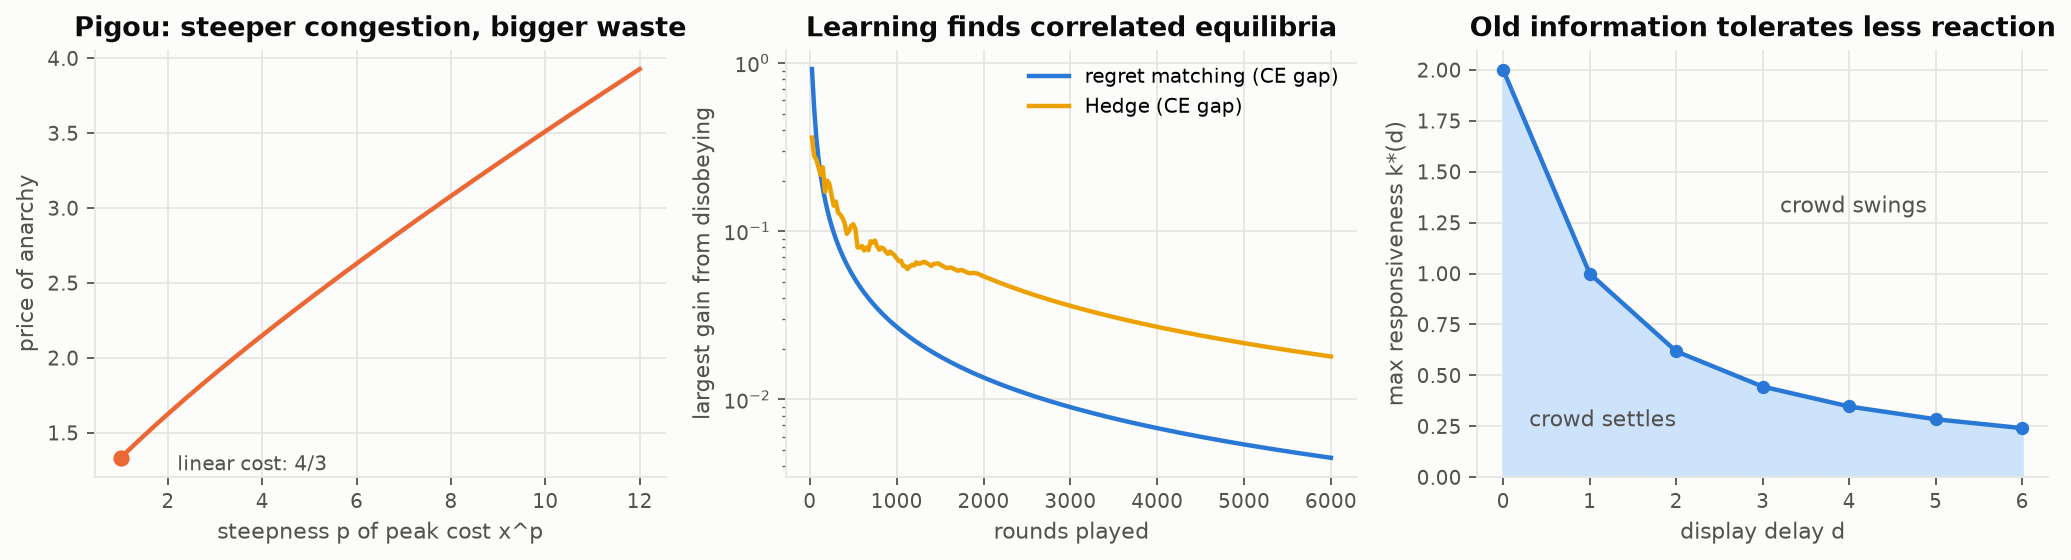
\includegraphics[width=\linewidth]{e0_theory.png}
\vspace{-1.6em}\caption{Theory. Left: PoA of Pigou's network grows with steepness. Middle: in the intersection game,
regret matching drives the CE gap of the empirical play to zero; Hedge reaches the coarse CE set. Right: stability
limit $k^*(d)$ for $y_{t+1}=y_t-k\,y_{t-d}$ (matches the numeric root analysis to $10^{-6}$).}\label{fig:theory}\end{figure}

\textbf{RQ1: what selfish timing costs.} Table~\ref{tab:poa} and Fig.~\ref{fig:poa}. A normal dinner loses
1.81\,min per student (PoA 6.7) and a special dinner 7.57\,min (PoA 4.6). Across the four messes this is
\textbf{132 student-hours per normal day}. Normal breakfasts have no queue at all. The planner removes waiting
entirely by feeding arrivals at exactly the serving rate, at the price of moving some students one or two slots.
The bumpy Nash profile is genuine: the slot right after a rush inherits its backlog, so arriving at the start of a
rush is better than just after it. The same 3--8$\times$ gap appears in every domain, and Pigou's 4/3 is recovered
exactly when the slot model uses linear costs (unit test).

\begin{table}[H]\centering\small
\caption{Selfish (Nash) vs.\ planner, minutes per person (mess rows: average of 4 messes). Last three columns (Prop.~\ref{p3}): share of people tempted to disobey the optimum, average obedience reward per person, and time saved per person vs.\ Nash.}\label{tab:poa}
\begin{tabular}{lrrrrrr}\toprule
Instance & Nash & Optimum & PoA & Tempted & Reward & Saving\\\midrule
Mess lunch, normal / special & 1.39 / 4.87 & 0.21 / 1.25 & 6.7 / 3.9 & & & \\
Mess dinner, normal / special & 2.14 / 9.71 & 0.33 / 2.14 & 6.7 / 4.6 & & & \\\midrule
Road: bridge commute (2400 cars) & 17.12 & 4.50 & 3.8 & 52\% & 4.48 & 12.62\\
Network: night backups (600 jobs) & 3.71 & 1.13 & 3.3 & 56\% & 1.09 & 2.58\\
Restaurant: food court (450) & 2.35 & 0.50 & 4.7 & 20\% & 0.48 & 1.85\\
Gym: evening (240) & 1.68 & 0.31 & 5.4 & 13\% & 0.27 & 1.37\\
Mess dinner, generic (680) & 2.21 & 0.28 & 8.0 & 11\% & 0.27 & 1.93\\\bottomrule
\end{tabular}\end{table}

\begin{figure}[t]\centering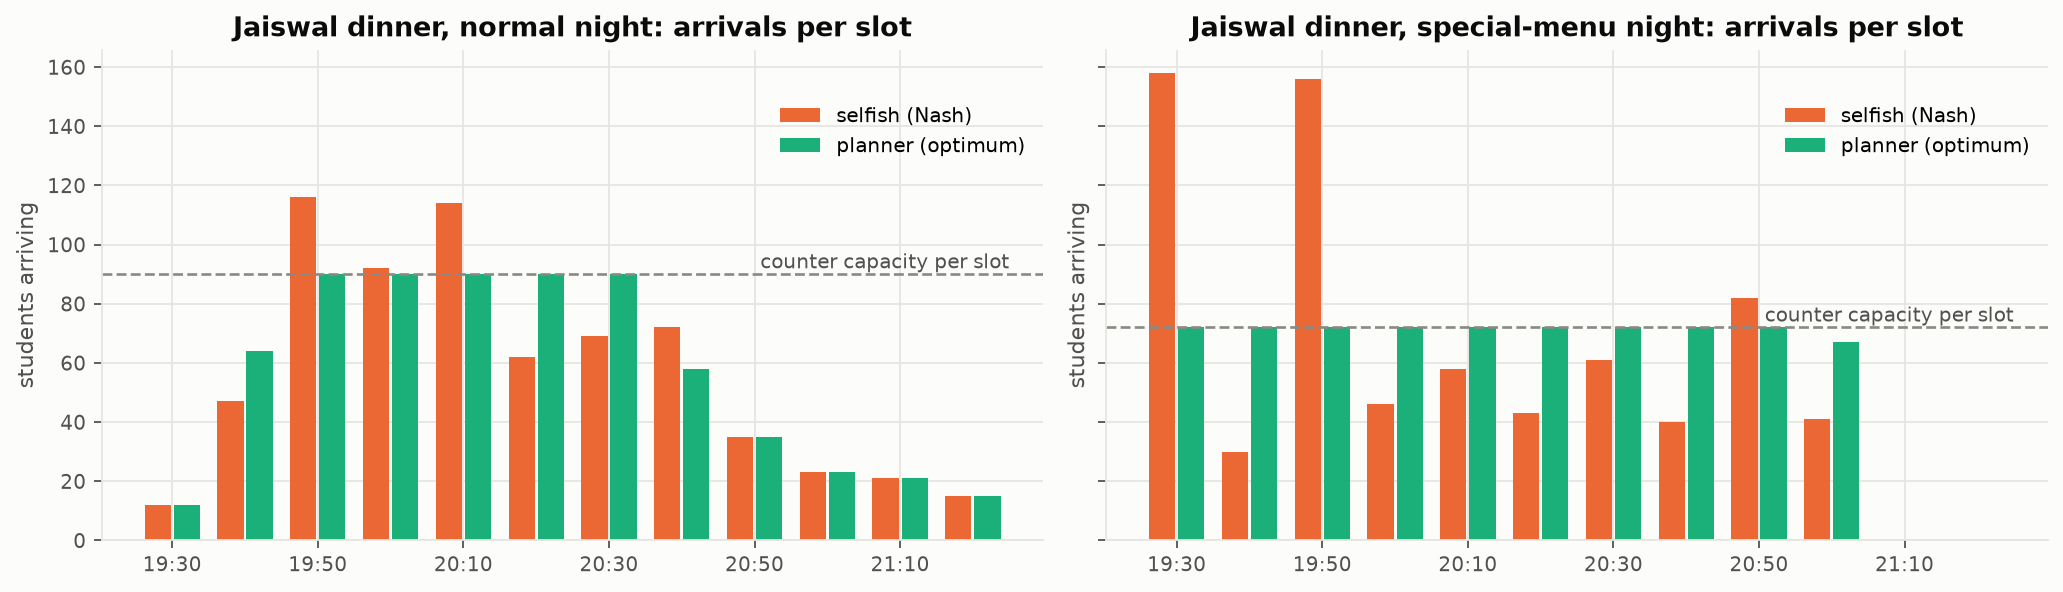
\includegraphics[width=\linewidth]{e2_nash_vs_optimum.png}
\vspace{-1.6em}\caption{Arrivals per slot at Jaiswal dinner: selfish (orange) overloads the counter (dashed); the
planner (green) smooths arrivals to capacity.}\label{fig:poa}\end{figure}

\textbf{RQ2: what the display should show.} Fig.~\ref{fig:pol}. \emph{More information can be worse.} For a
reactive crowd the exact live counter raises the cost from 2.24 (Nash) to \textbf{11.55\,min}, with 76\% of the
crowd switching slots each day: the rush jumps around, as in the two-student game. Coarse levels do not help
(12.95), and private noise helps partly (6.94 at sd 3 and 3.2 at sd 8, Fig.~\ref{fig:sweeps}). Showing the counter
to at most half the crowd costs almost nothing (2.11--2.16), whereas showing it to 70\% raises the cost to 4.95:
\textbf{H1 holds for a reactive crowd}. For calm crowds no information is cheapest (1.65), but only because people
keep pessimistic memories. Their positive regret (0.37\,min) means the outcome lasts only while they never learn.
\textbf{H2 (delay).} With 30\% of people reacting daily the swing grows from 2\% (delay 1) to 11\% (delay 4)
(Fig.~\ref{fig:sweeps}), as predicted by $k^*(d)$ shrinking with $d$.

\begin{figure}[t]\centering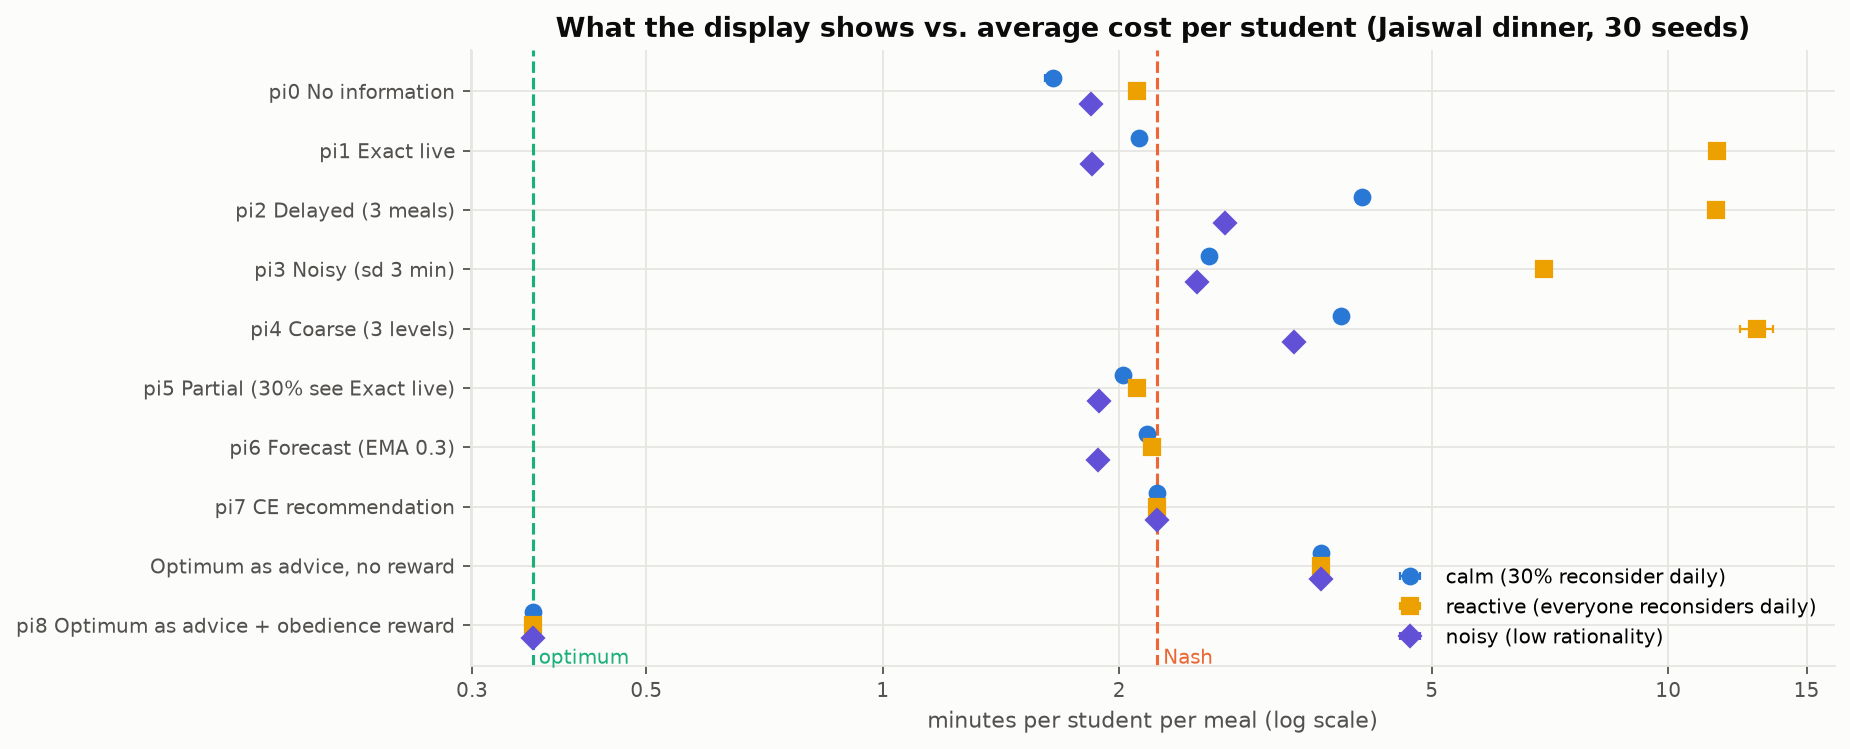
\includegraphics[width=0.93\linewidth]{e3_policies.png}
\vspace{-0.8em}\caption{Average cost under each policy and behaviour regime (Jaiswal dinner, 30 seeds, 95\% CI; log
scale). The CE recommendation ($\pi_7$) gives the same result in every regime; only $\pi_8$ reaches the optimum.}\label{fig:pol}\end{figure}

\begin{figure}[t]\centering
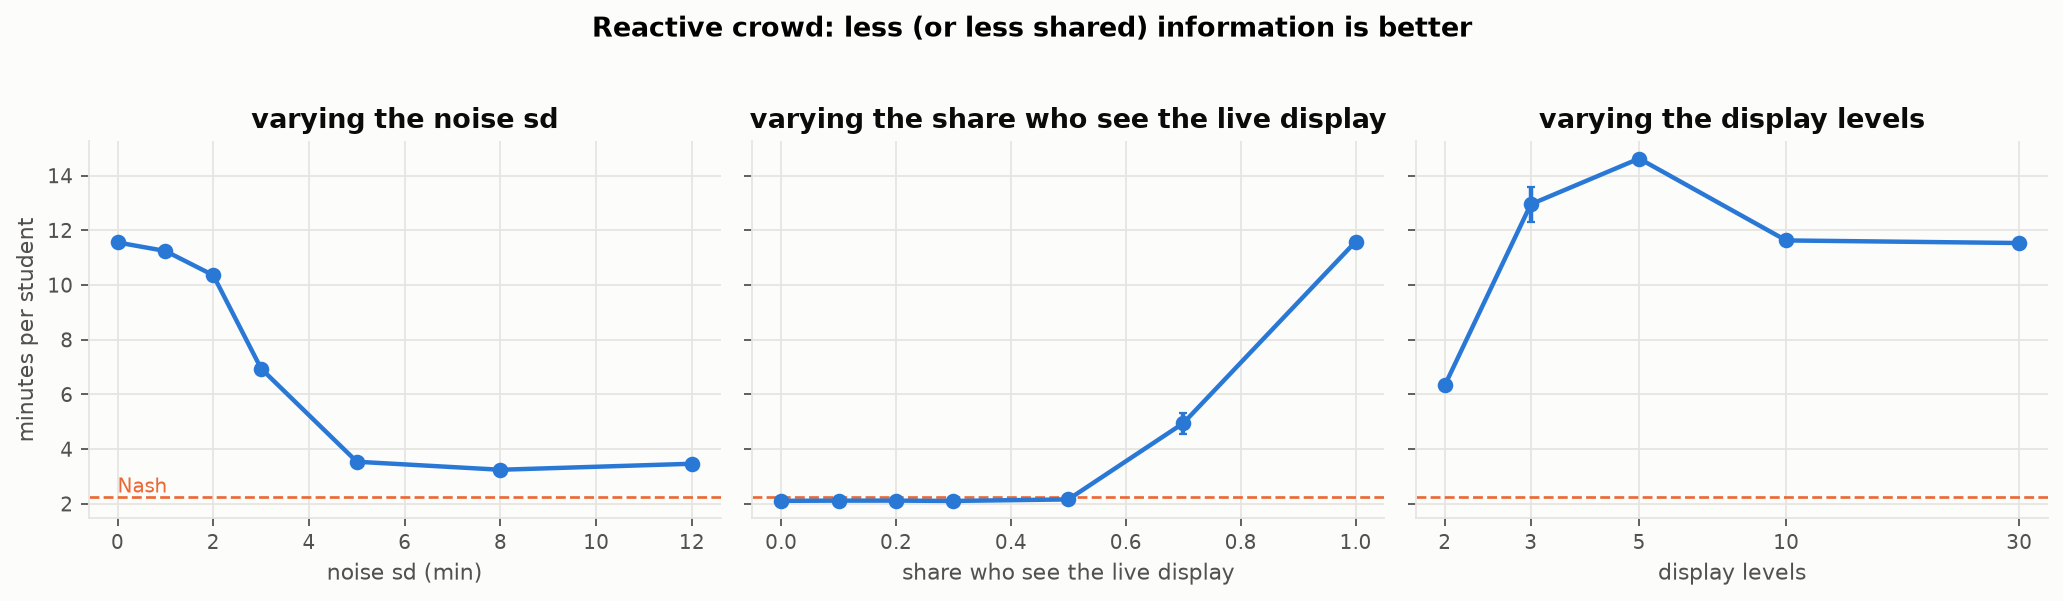
\includegraphics[width=\linewidth]{e4_sweeps.png}\\[2pt]
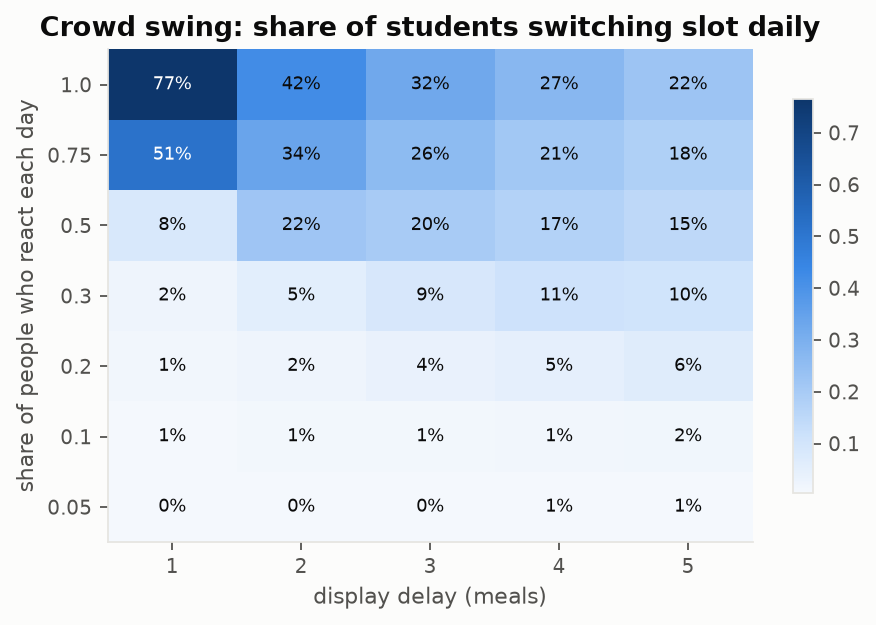
\includegraphics[width=0.48\linewidth]{e5_delay_swing.png}
\vspace{-0.6em}\caption{Top: reactive crowd, cost vs.\ private noise, share of viewers and number of display levels
(dashed: Nash). Bottom: crowd swing vs.\ display delay and share of people reacting daily.}\label{fig:sweeps}\end{figure}

\textbf{RQ3: correlated recommendations.} Fig.~\ref{fig:ce}. The Nash-based recommendation is a CE: nobody gains by
disobeying (0.0\,s at Jaiswal dinner). Its outcome is the same in all three regimes, with zero swing and zero regret.
With the live display as the fallback for non-users, it removes the herding of a reactive crowd once 50\% (2.53)
to 70\% (2.12) of students use it. The optimum, by contrast, is \emph{not} a CE: 13\% of students would gain up to
2.9\,min by disobeying, and when rational students do disobey the cost \emph{rises} to 3.61. The best-CE LP over 26
schedules returns exactly the Nash cost (2.235), and so does the best CCE, confirming Prop.~\ref{p2}: advice
coordinates but cannot make people accept worse slots for others. Prop.~\ref{p3} closes the gap. Rewarding the
13\% sent off-peak with about 2.7 minutes' worth of priority (0.35\,min per student on average) makes the optimum
self-enforcing ($\pi_8$: \textbf{0.36\,min}, a 6$\times$ reduction). \textbf{H3 is refined}: recommendations close the
NE--optimum gap only together with obedience rewards.

\begin{figure}[t]\centering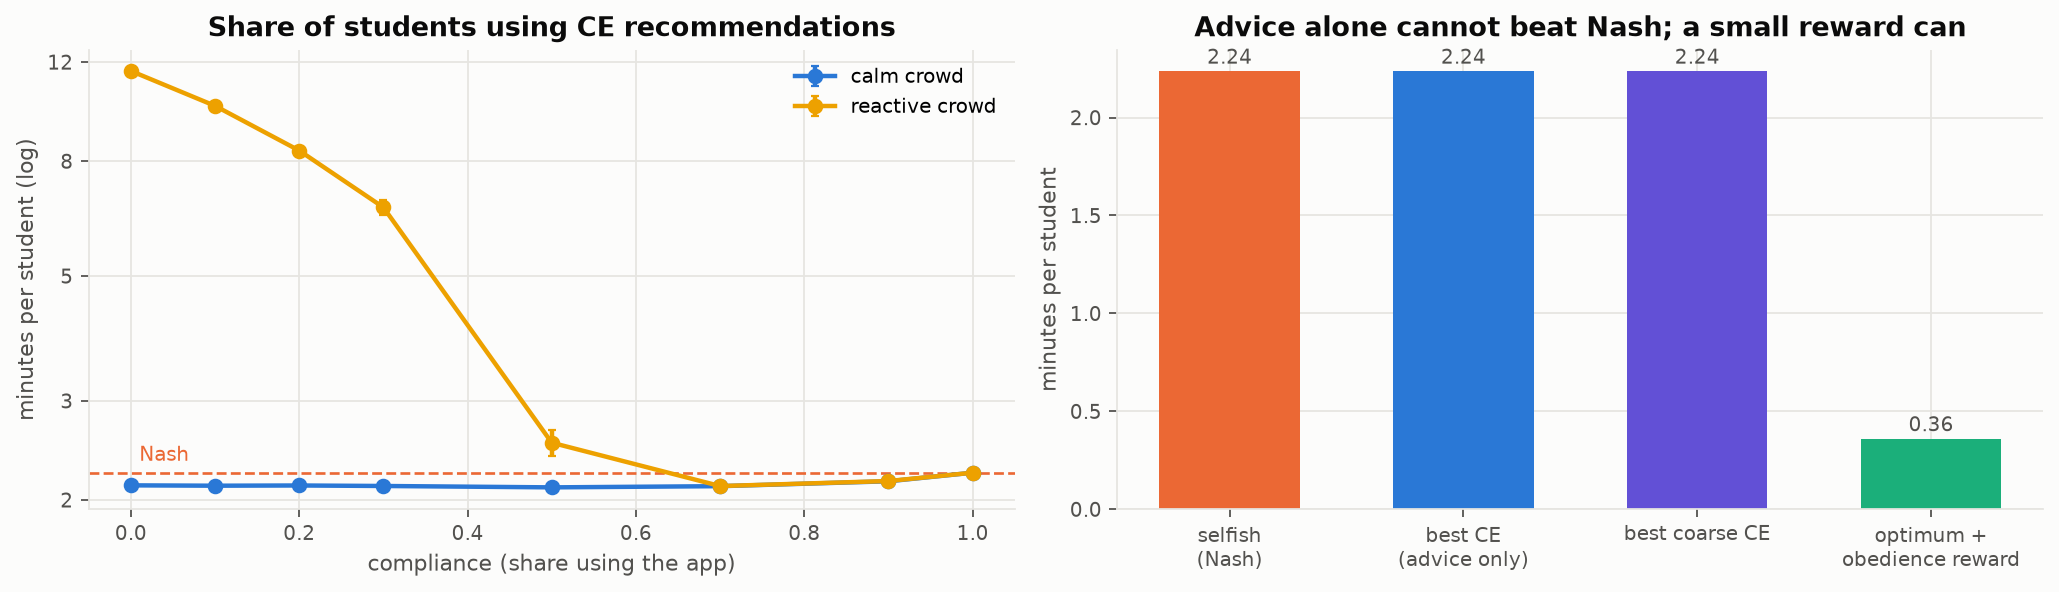
\includegraphics[width=\linewidth]{e6_correlated.png}
\vspace{-1.6em}\caption{Left: share of students using CE recommendations (non-users see the live display). Right:
advice alone (best CE / CCE from the LP) equals Nash; the optimum with the obedience reward is 6$\times$ cheaper.}\label{fig:ce}\end{figure}

\textbf{Learning, incomplete information, data.} With published waits, Hedge and regret matching settle near Nash
(2.29 / 2.31\,min). Their swap regret falls to 0.19 / 0.03\,min per day, i.e.\ joint play approaches a CE, as theory
predicts. EXP3, which only sees its own wait, still has 5.1\,min of regret after 300 days: publishing data helps
learning (Fig.~\ref{fig:learn}). In the Bayesian analysis (slow night with probability 0.3, counter at 70\%),
announcing the night lowers the expected cost from 4.47 to 3.37 (+1.10\,min per student). On \emph{normal} nights,
however, it raises the cost from 0.88 to 2.24, because the fear of a slow night was keeping people spread out.
Calibration from scans alone recovers $\mu$ within 2--3\% whenever queues form (it is only a lower bound when they
never do), and recovers preferred slots for 97\% of students within one slot at dinner (Table~\ref{tab:data}).

\begin{figure}[t]\centering
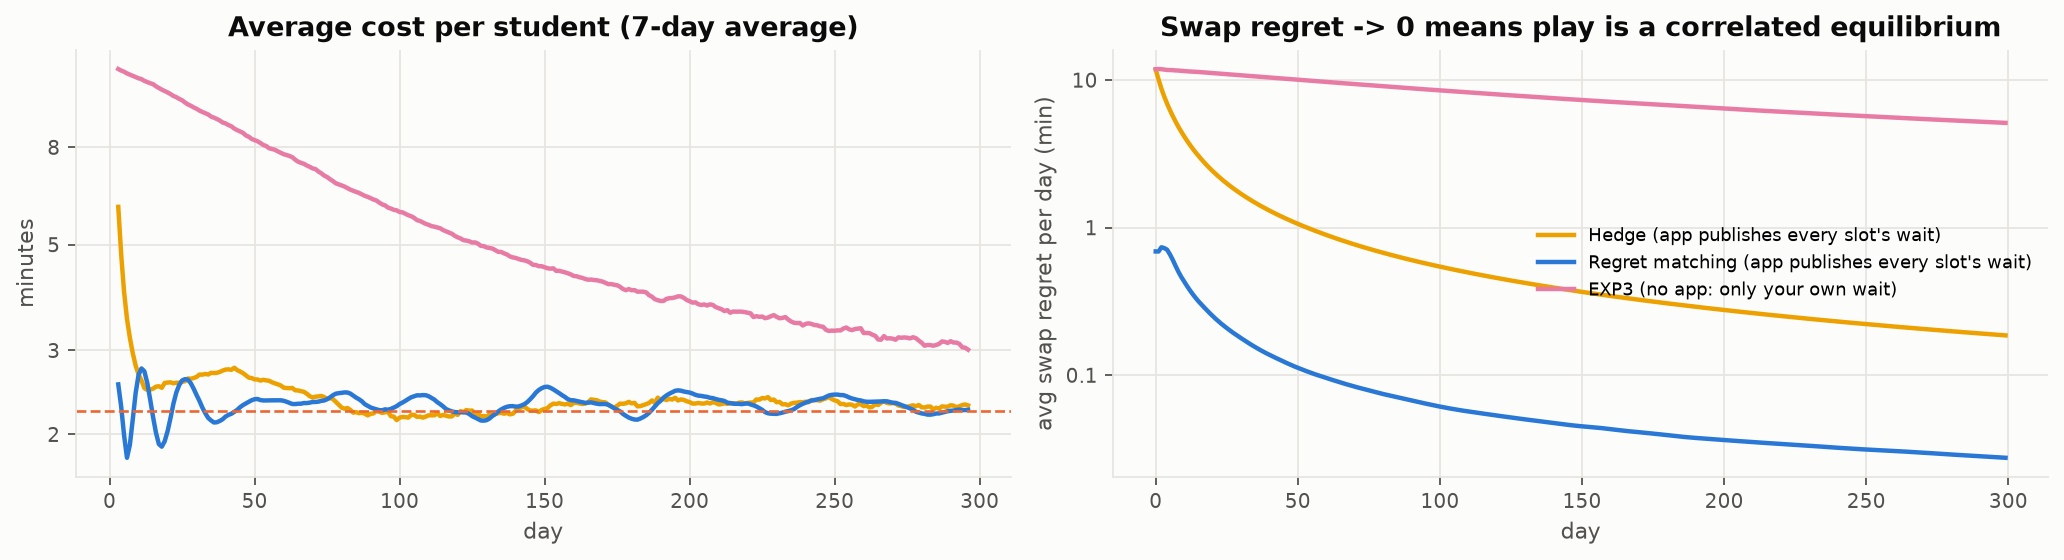
\includegraphics[width=\linewidth]{e7_learning.png}\\[2pt]
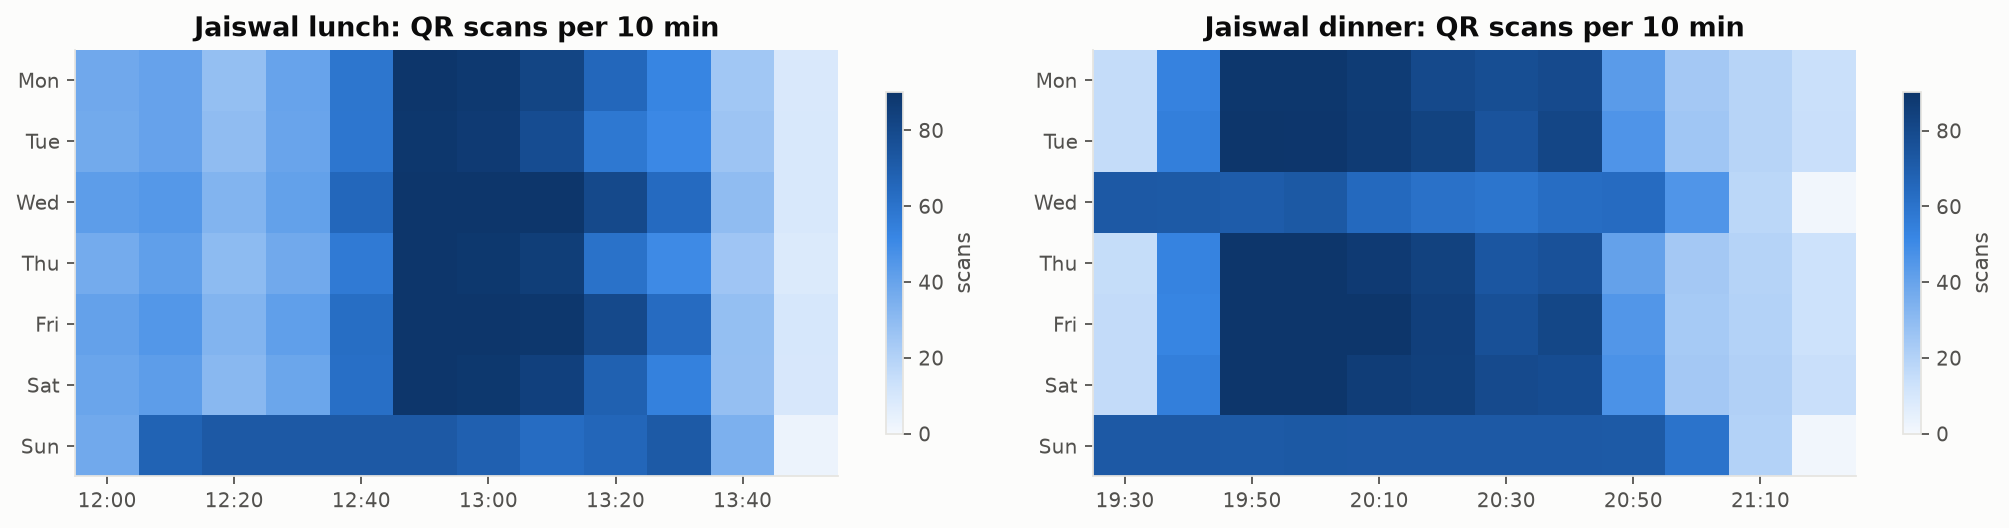
\includegraphics[width=\linewidth]{e1_heatmap.png}
\vspace{-1.4em}\caption{Top: learning over 300 days (dashed: Nash). Bottom: synthetic QR scans per 10 minutes by
weekday; the plateaus are the serving rate (Sunday lunch, Wednesday and Sunday dinner are special).}\label{fig:learn}\end{figure}

\begin{table}[H]\centering\small
\caption{Learning unknowns from the scan logs (Jaiswal; nowcast MAE averaged over 4 messes, scans per 10-min slot).}\label{tab:data}
\begin{tabular}{lccccc}\toprule
Meal, menu & true $\mu$ & estimated $\mu$ & mean scans/slot & N0 MAE & N1 MAE\\\midrule
Breakfast, normal & 8.0 & 6.2 (no queue: lower bound) & 28.2 & 3.89 & \textbf{3.38}\\
Breakfast, special & 6.4 & 6.6 & 30.1 & \textbf{3.64} & 3.74\\
Lunch, normal & 9.0 & 9.2 & 39.8 & \textbf{4.02} & 4.05\\
Lunch, special & 7.2 & 7.4 & 43.7 & \textbf{3.36} & 3.56\\
Dinner, normal & 9.0 & 9.2 & 42.3 & \textbf{4.41} & 4.58\\
Dinner, special & 7.2 & 7.4 & 43.4 & 4.37 & \textbf{3.63}\\
\bottomrule\end{tabular}\end{table}
\vspace{-0.4em}
\noindent\textbf{RQ4: nowcasting.} Both forecasters predict the next 30 minutes within 8--14\% of the mean load.
Scaling by tonight's scans (N1) helps most when an evening starts unusually (normal breakfasts $-13\%$, special
dinners $-17\%$); elsewhere the two are within 5\%, as the extra information in a few early scans is offset by their
noise. Preferred slots are recovered exactly for 80\% of students at dinner (97\% within one slot).

% ============================================================================
\section{Limitations and future work}
All data are synthetic, so the conclusions are about mechanisms (herding, obedience, the price of obedience), not
exact IITGN minutes. The fluid queue spreads arrivals evenly, so the optimum's zero wait (and hence the PoA) is
optimistic. With carry-over the game has no potential, so we report $\varepsilon$-equilibria (at most 14\,s). The
optional scarcity penalty makes the game lumpier ($\varepsilon$ up to about 2\,min), so it is off by default. Behaviour
models are assumptions, and we report which conclusions change across them. Future work: a Telegram bot pilot in one
mess; dosa tokens or pre-booked slots as non-monetary tolls; choice between messes (a routing game, where Braess
effects are possible); differentially private displays; and a second scan at the queue entrance to measure waits.

% ============================================================================
\needspace{18\baselineskip}
\section{Contribution}
The work was split into four packages, one per member, following the plan in our project brief. All four members
took part in the modelling decisions, the analysis of results and the writing of this report.
\begin{table}[H]\centering\small
\caption{Work packages, what each member delivered (files in \texttt{crowd/} and experiments), and status.}\label{tab:contrib}
\begin{tabular}{>{\raggedright\arraybackslash}p{2.3cm}>{\raggedright\arraybackslash}p{10.6cm}>{\raggedright\arraybackslash}p{2.3cm}}\toprule
Member & Work package and deliverables & Status\\\midrule
Harsh Kumar Jha & \textbf{Data and case study.} Mess scenario (4 messes, 3 meals, special menus), synthetic roster
and QR-scan logs, serving-rate and preference calibration, nowcasting N0/N1 (\texttt{mess.py}; E1, E9). &
\textbf{Fulfilled}$^{a}$\\
Yash Goyal & \textbf{Incomplete information, learning and statistics.} Bayesian game and value of information;
Hedge, EXP3 and regret-matching learners; 30-seed confidence intervals; Streamlit demo, README and repository
(\texttt{correlated.py}, \texttt{simulate.py}, \texttt{app.py}; E7, E8). & \textbf{Fulfilled}\\
Piyush Kumar Keshri & \textbf{Equilibria and correlated equilibrium.} Toy games; NE, CE and CCE linear programs;
Nash, Wardrop and optimum solvers; price of anarchy; CE recommender, Propositions 1--3, best-CE LP and obedience
reward (\texttt{theory.py}, \texttt{game.py}, \texttt{correlated.py}; E0, E2, E6). & \textbf{Fulfilled} (extended with $\pi_8$)\\
Garv Singhal & \textbf{Simulator and information policies.} Day-to-day simulator, policies $\pi_0$--$\pi_8$, behaviour
regimes, sweeps, delay and crowd-swing analysis, generic domains (\texttt{simulate.py}, \texttt{domains.py};
E3--E5). & \textbf{Fulfilled}\\\bottomrule
\end{tabular}

\vspace{2pt}\raggedright\footnotesize $^{a}$As agreed with our advisor, real scan logs were replaced by a synthetic
semester, and the manual queue-timing study by the generator's ground-truth waits.
\end{table}
{\sloppy\noindent\textbf{Reproducibility:}
\texttt{pip install -r requirements.txt; pytest -q} (54 checks); \texttt{python experiments.py} regenerates every
figure and number in this report (\texttt{results/RESULTS.md}); \texttt{streamlit run app.py} opens the demo, which is also hosted at \url{https://crowd-congestion.streamlit.app/}.\par}

\begin{thebibliography}{99}\small\setlength{\itemsep}{0pt}
\bibitem{arthur} W.~B.~Arthur. Inductive reasoning and bounded rationality. \emph{AER}, 84(2):406--411, 1994.
\bibitem{aumann} R.~J.~Aumann. Subjectivity and correlation in randomized strategies. \emph{J.\ Math.\ Econ.}, 1(1):67--96, 1974.
\bibitem{nash} J.~F.~Nash. Equilibrium points in n-person games. \emph{PNAS}, 36(1):48--49, 1950.
\bibitem{rosenthal} R.~W.~Rosenthal. A class of games possessing pure-strategy Nash equilibria. \emph{IJGT}, 2:65--67, 1973.
\bibitem{koutsoupias} E.~Koutsoupias, C.~Papadimitriou. Worst-case equilibria. \emph{STACS}, 404--413, 1999.
\bibitem{roughgarden} T.~Roughgarden, \'E.~Tardos. How bad is selfish routing? \emph{J.\ ACM}, 49(2):236--259, 2002.
\bibitem{harsanyi} J.~C.~Harsanyi. Games with incomplete information played by ``Bayesian'' players, I--III. \emph{Mgmt.\ Sci.}, 14(3):159--182, 1967.
\bibitem{mckelvey} R.~D.~McKelvey, T.~R.~Palfrey. Quantal response equilibria for normal form games. \emph{GEB}, 10(1):6--38, 1995.
\bibitem{freund} Y.~Freund, R.~E.~Schapire. A decision-theoretic generalization of on-line learning. \emph{JCSS}, 55(1):119--139, 1997.
\bibitem{auer} P.~Auer, N.~Cesa-Bianchi, Y.~Freund, R.~E.~Schapire. The nonstochastic multiarmed bandit problem. \emph{SICOMP}, 32(1):48--77, 2002.
\bibitem{hart} S.~Hart, A.~Mas-Colell. A simple adaptive procedure leading to correlated equilibrium. \emph{Econometrica}, 68(5):1127--1150, 2000.
\bibitem{vickrey} W.~S.~Vickrey. Congestion theory and transport investment. \emph{AER}, 59(2):251--260, 1969.
\end{thebibliography}
\end{document}
